\documentclass[border=3mm]{standalone}
\usepackage{tikz}
\usetikzlibrary{shapes.geometric}
\colorlet{pagebackground}{yellow!10}
\pagecolor{pagebackground}
\begin{document}
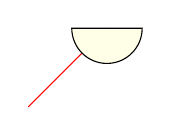
\begin{tikzpicture}
  \coordinate (a) at (1,1);
  \draw [red](0,0) -- (a);
  \node [semicircle,draw,shape border rotate=180,anchor=chord center,outer sep=0cm,inner sep=0.2cm,fill=pagebackground] at (a) {};
\end{tikzpicture}
\end{document}